\section{Simulation}
Une difference etre les tube photomultiplicateur et les SiPM est que les tube photomultiplicateur ont une zone de detection en forme de rond alors que les SiPM ne peuve que etre produit en carré et donc les une zone de detection carré. Cela implique donc un changement de forme de cristal. Pour s'assurer que les ancien cristaux et les nouveaux se comporte de la meme maniere, nous allons faire une simulation. Les cristaux NaI utiliser actuelment sont des cylindre de 28mm de diametre et 50mm de hauteur. Pour que les nouveaux critaux cuboide rentre dans le boitier, ils doive avoir une longeur et une largeur de 20mm et pour que le volume, et donc normalement le nombre de detection, reste le meme, ils doive avoir une hauteur de 76.96mm. Nous testeron egalement un cristal avec un hauteur de 75mm pour voir si la petit difference de volume a un impact sur les resultats.
\begin{figure}
    \centering
    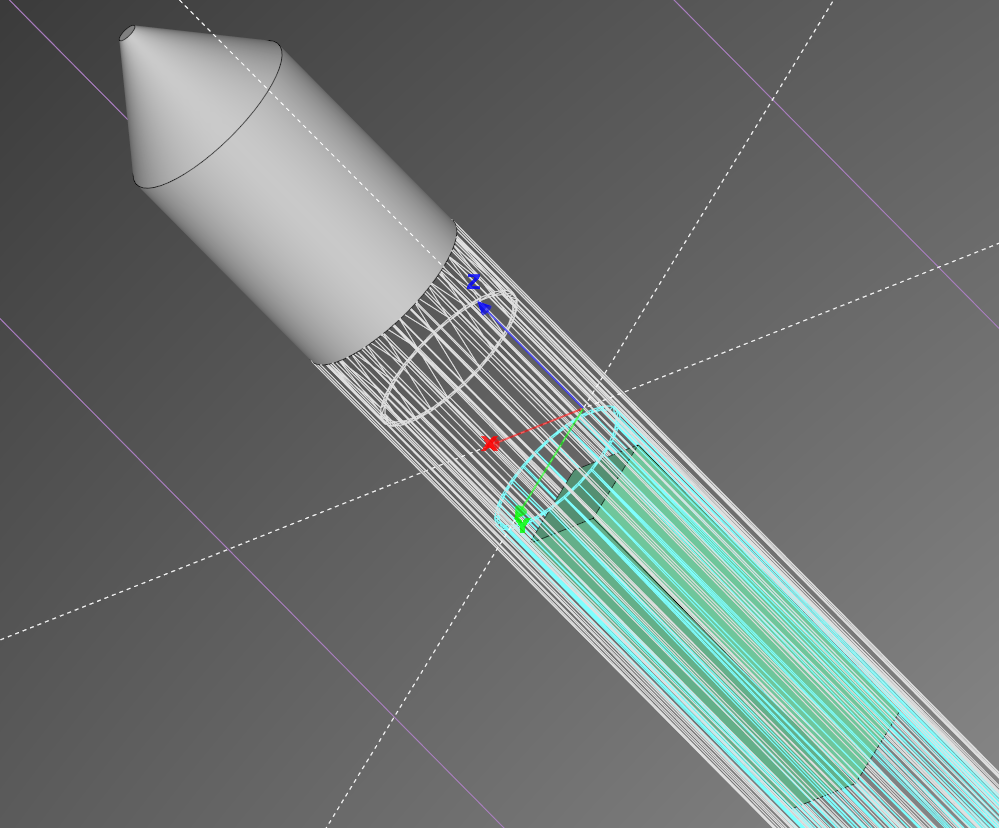
\includegraphics[width=0.5\textwidth]{photo/sonde_carre_simu.PNG}
\end{figure}

Un autre stagiare travailler sur des sujet de simulation et a donc pu faire ces simulation pour moi. 